%!TEX root = ../thesis.tex
\setchapterpreamble[ur][.9\textwidth]{%
\dictum[Dr. Zefram Cochrane, Entwickler des Warp-Antriebs \\ aus ``Star Trek: Enterprise – Broken Bow: Part 1'']{%
``On this site, a powerful engine will be built - an engine that will someday help us to travel a hundred times faster than we can today. [...] This engine will let us go boldly, where no man has gone before.''}
}

\chapter{WARP – Eine Webanwendung für Build- und Deployment-Prozesse}

Die Benennung einer Anwendung ist generell für die Entwicklung irrelevant. Als Entwickler legen wir im Vorfeld trotzdem gerne einen Namen für unsere Software fest – wenigstens einen vorläufigen Projektnamen – um die Benennung verschiedenster Dinge zu erleichtern: u.a. Namensräume, interne Bibliotheken, Projekte auf GitHub \& Co.

Der Projektname \textbf{WARP} wurde bei Präsentationen meist direkt mit der Science-Fiction Fernsehserie \emph{Star Trek} in Verbindung gebracht. Der Ursprung des Namens liegt jedoch nicht bei der Reise durch das All, sondern bei Nintendos Super Mario.

\begin{figure}[H]
  \caption{Warp Pipes in Super Mario Bros.}
  \label{fig:super-mario-warp-pipes}
  \centering
    
\includegraphics[width=.5\textwidth]{assets/mario-pipes}
  \floatfoot{Copyright Nintendo 1985, Quelle: www.nintendo.de}
\end{figure}

Die Warp Pipes aus der Super Mario Franchise befördern unseren Pro\-ta\-go\-nisten Mario von einem Ende der Röhre an das andere Ende, welches sich weit entfernt, vielleicht auch in anderen Welten befindet. Letztendlich ist die Assoziation durch die Analogie der Rohrleitung \emph{(Pipeline)} entstanden, welche auch als Begriff in Deployment Prozessen auftauchen.

Dieses Kapitel beinhaltet den kompletten Entwurf und die Implementierung der Anwendung \textbf{WARP}. Zuerst wird ein genereller Überblick über verschiedene Aspekte der Anwendung gegeben, die zum weiteren Verständnis notwendig sind. Darauf folgen Details des Services und des Clients. Da Service und Client zwei abgegrenzte Teile sind (inhaltlich und technisch), wird jeweils einzeln auf Entwurf und Implementierung eingegangen.

\section{Architekturentwurf}

Die Webanwendung ist im Client-Server-Modell umgesetzt, wobei der Server eine API besitzt und im weiteren Verlauf als Service bzeichnet wird. Im Folgenden wird die grundlegende Architektur der Anwendung kurz beschrieben. Abbildung \ref{fig:architektur} zeigt eine grafische Übersicht über die Bestandteile des Systems und deren Beziehungen.

\begin{figure}[h]
  \caption{Architektur der Anwendung}
  \label{fig:architektur}
  \centering
    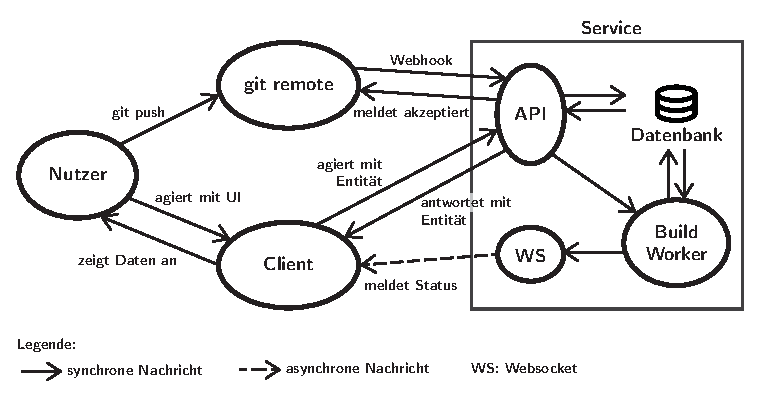
\includegraphics[width=\textwidth]{assets/systemarchitektur}
\end{figure}

\subsection{Übersicht über die Anwendung}
\label{subsec:uebersicht-anwendung}

Der Service ist für das Persistieren und Verwalten von Daten zuständig. Zum Abfragen und Verändern von Daten bietet der Service eine \ac{API} an. Ebenso startet der Service auf Anfrage einen Build Prozess.

Ein Build Prozess wird gestartet, indem eine bestimmte URL über einen Git Webhook aufgerufen wird. Der Git Webhook wird so konfiguriert, dass jene URL nach jedem Push auf den Git Remote aufgerufen wird.

Der Webhook übermittelt im Body des HTTP-Requests nützliche Informationen, darunter auch Daten über den letzten Commit und die Git Reference. Mit diesen Daten kann somit ein passender Build Prozess erstellt und gestartet werden.

Während des Build Prozesses wird der aktuelle Status in Echtzeit an alle verbundenen Clients gesendet.

Der Client zeigt letztendlich alle Daten. Über seine Oberfläche hat der Nutzer die Möglichkeit, verschiedene \ac{CRUD} Aktionen auszuführen.

\subsection{Datenstruktur}
\label{subsec:uml}

Abbildung \ref{fig:uml} zeigt die Datenstruktur der Anwendung.

Eine Pipeline besitzt beliebig viele Builds als Instanz einer Pipeline. Ein Build ist einem Commit des im Projekt definierten Git Repositories zugeordnet. Dadurch ist für den Nutzer später schneller ersichtlich, welcher Stand einem Build zugrunde liegt.

Wie in CHAPREF DEFINITIONEN bereits definiert wurde, besteht ein Build aus mehreren Stages, die nacheinander ausgeführt werden. Im Datenmodell (Abbildung \ref{fig:uml}) wurde die Stage jedoch als \emph{Abschnitt} generalisiert. Ein solcher Abschnitt besitzt einen Ausführungstyp, welcher festlegt, ob die Kinder eines Abschnittes parallel oder seriell ausgeführt werden sollen. Der Abschnitt besitzt entweder weitere Abschnitte oder Schritte als Kinder. Somit ist eine Stage eine bestimmte Instanz eines Abschnittes, deren Ausführungstyp immer seriell ist. Dies macht eine Generalisierung sinnvoll.

Ein \emph{Schritt} ist die kleinste Einheit des Build-Prozesses. Er besitzt neben den Attributen des Abschnittes auch den auszuführenden Befehl und ein Feld für die Ausgabe (Log). Alle Schritte zusammen ergeben den gesamten Build-Prozess, dessen Abfolge über Abschnitte festgelegt ist.

\begin{figure}[h]
  \caption{UML Diagramm der Anwendung}
  \label{fig:uml}
  \centering
    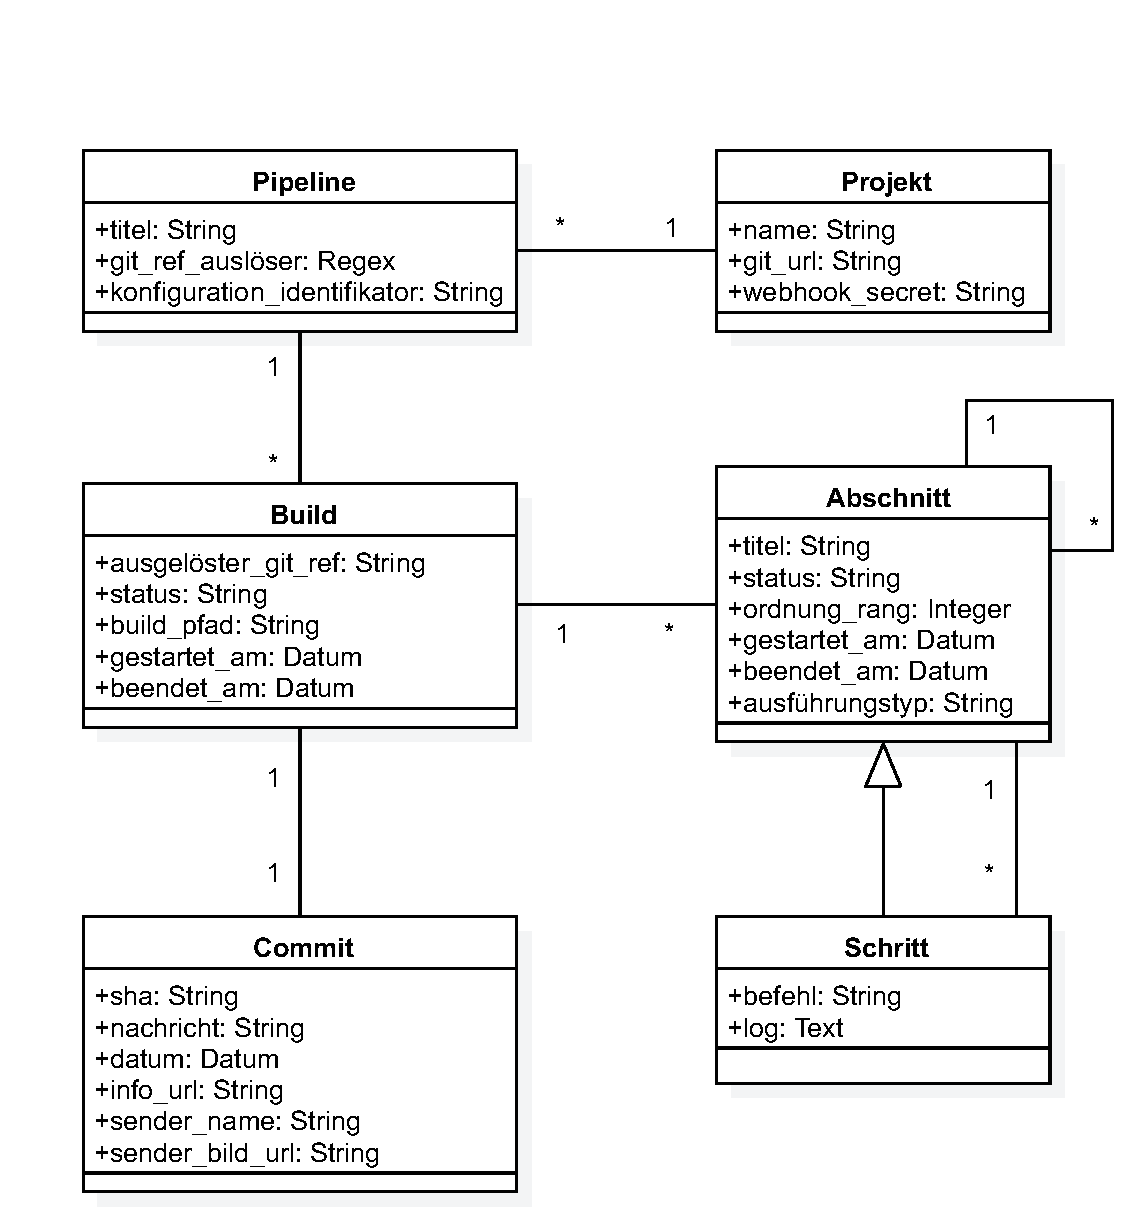
\includegraphics[width=\textwidth]{assets/uml}
\end{figure}
